\documentclass[
    11pt,
    a4paper,
    egregdoesnotlikesansseriftitles,
    toc=chapterentrywithdots,
    openany,
    oneside,
    titlepage,
    parskip=half,
    headings=normal,  % reduces heading size
    listof=totoc,
    bibliography=totoc,
    index=totoc,
    captions=tableheading,  % caption below table
    chapterprefix,
    listof=flat,
    final
]{scrbook}


% details about your thesis
\newcommand{\titel}{Koroutine, Threads und Asyncio}
\newcommand{\artderarbeit}{Studienarbeit}  % {Bachelorarbeit,Masterarbeit}
\newcommand{\autor}{Christoph Kirschner}
\newcommand{\studiengang}{FWPM Skriptsprache Python}  % {Informatik,Wirtschaftsinformatik,Medieninformatik}
\newcommand{\matrikelnr}{3248161}
\newcommand{\ausgabe}{23.09.2021}
\newcommand{\abgabe}{03.10.2021}
\newcommand{\erstgutachter}{Prof. Dr.-Ing. Jürgen Krumm}
\newcommand{\zweitgutachter}{Prof. Dr. Matthias Wieczorek}
\newcommand{\logo}{figures/TH-Nuernberg-RGB.png}
\newcommand{\keywords}{hot, fuzz}
 

% custom head and foot
\usepackage[automark]{scrlayer-scrpage}
\pagestyle{scrheadings}
\ihead{\headmark}
\chead{}
\ohead{\pagemark}
\renewcommand*\chaptermarkformat{\chapappifchapterprefix{\ }% 
  \thechapter.\enskip}

\usepackage{titlesec}


\RedeclareSectionCommand[tocindent=0pt]{section}
\RedeclareSectionCommand[tocindent=0pt]{subsection}
\RedeclareSectionCommand[tocnumwidth=30pt, beforeskip = -30pt]{chapter}


\usepackage{scrhack}

% other packages
\usepackage[utf8]{inputenc}
\usepackage[T1]{fontenc}
\usepackage{lmodern,relsize,textcomp,csquotes}
\usepackage{amsmath,amsfonts}
\usepackage[ngerman,ngerman]{babel}  % flip for German thesis
\usepackage[final]{graphicx}
\usepackage{setspace,geometry,xcolor}
\usepackage{makeidx}
\usepackage{paralist,ifthen,todonotes}
\usepackage{url}
%\usepackage[toc]{glossaries}
\usepackage{pdfpages}
\usepackage[style = numeric, backend = bibtex]{biblatex}


% table setup
\usepackage{longtable}
\usepackage{array}
\usepackage{ragged2e}
\usepackage{lscape}

% pdf hyperref
\usepackage[
    bookmarks=true,
    bookmarksopen=true,
    bookmarksnumbered=true,
    bookmarksopenlevel=1,
    pdftitle={\titel},
    pdfauthor={\autor},
    pdfcreator={\autor},
    pdfsubject={\titel},
    pdfkeywords={\keywords},
    pdfpagelabels=true,
    colorlinks=true,
    linkcolor=red,
    urlcolor=magenta,
    anchorcolor=black,
    citecolor=cyan,
    filecolor=magenta,
    menucolor=red,
    plainpages=false,
    hypertexnames=true,
    linktocpage=true,
]{hyperref}


% configure your listings style
\usepackage{listings}
\lstset{
	tabsize=3,
	extendedchars=true,
	frame=single,
	showstringspaces=true,
	numbers=left,
	numberstyle=\small,
	breakautoindent=true,
	basicstyle=\small
}

\renewcommand{\lstlistingname}{Auflistung} % Aendert Listing zu Auflistung
\renewcommand{\lstlistlistingname}{Auflistungsverzeichnis} % Aendert Listing zu Auflistung

% page setup
% \setlength{\topskip}{\ht\strutbox}
\geometry{paper=a4paper,left=3cm,top=2cm,right=2cm,bottom=2cm}
\onehalfspacing
\frenchspacing
\clubpenalty = 10000
\widowpenalty = 10000 
\displaywidowpenalty = 10000

% some commands
\newcommand{\ua}{\mbox{u.\,a.\ }}
\newcommand{\zB}{\mbox{z.\,B.\ }}
\newcommand{\dahe}{\mbox{d.\,h.,\ }}
\newcommand{\bzw}{\mbox{bzw.\ }}
\newcommand{\bzgl}{\mbox{bzgl.\ }}
\newcommand{\eg}{\mbox{e.\,g.\ }}
\newcommand{\ie}{\mbox{i.\,e.\ }}
\newcommand{\wrt}{\mbox{w.\,r.\,t.\ }}
\newcommand{\etal}{\mbox{\emph{et.\,al.\ }}}

% load glossary entries
%\makenoidxglossaries
%\loadglsentries{glossary}

%\bibliographystyle{ieeetran}
\bibliography{refs_new}
\nocite{*}

\begin{document}

\setcounter{secnumdepth}{3}  % numerate subsections
\setcounter{tocdepth}{2}  % ...but don't include them in toc

\frontmatter
\thispagestyle{empty}
\pdfbookmark[1]{Cover}{cov}
\begin{titlepage}

\begin{center}


\includegraphics[width=\linewidth]{figures/TH-Nuernberg-RGB.png}\\[1cm]
\LARGE{Fakultät Elektrotechnik Feinwerktechnik Informationstechnik}\\[2cm]

\huge
\textbf{\titel}\\[1cm]
%
\Large
\artderarbeit~im \studiengang\\[1cm]
%
\large
vorgelegt von

\Large
\autor\\[0.5cm]
\small

\vspace*{\fill}

\large
\begin{tabular}{p{3cm}p{8cm}}\\
%Ausgabe:  & \quad \ausgabe\\[1.2ex]
Abgabe: & \quad \abgabe\\[1.2ex]
Prüfer:  & \quad \erstgutachter\\[1.2ex]
%discomment "Betreuer" and "Unternehmen" for a thesis in a company
%Betreuer: & \quad \betreuer\\
%Unternehmen: & \quad \unternehmen
\end{tabular}
\end{center}

\begin{center}
\copyright\,\the\year
\end{center}

\vspace{-0.5cm}
\singlespacing
\small

\end{titlepage}
\cleardoublepage

% download the following form and complete it (hit save in your editor)
% https://intern.ohmportal.de/fileadmin/Gelenkte_Doks/Abt/SZS/SB/%SB_0050_FO_Pruefungsrechtliche_Erklaerung_und_Erklaerung_zur_Veroeffentlichung_der_Abschlussarbeit_public.pdf

\includepdf{pruefungsrechtliche_erklaerung.pdf}\cleardoublepage

%\thispagestyle{empty}
\section*{Kurzdarstellung}
\label{sec:kurzdarstellung}
Kurze Zusammenfassung der Arbeit, höchstens halbe Seite.
Deutsche Fassung auch nötig, wenn die Arbeit auf Englisch angefertigt wird.

\blindtext


\section*{Abstract}
\label{sec:abstract}
\emph{Only if thesis is written in English.}

\blindtext
\cleardoublepage

%\titleformat{\chapter}
%  {\Large\bfseries} % format
%  {}                % label
%  {0pt}             % sep
%  {\huge}           % before-code
%  
\tableofcontents\cleardoublepage

\mainmatter
\chapter{Einleitung}
\label{ch:intro}

\chapter{Konzepte}
\label{ch:concept}

\section{Zielsetzung}
\label{sec:zielsetzung}
Wie bereits in Kapitel \ref{ch:intro} beschrieben, dient diese Projektarbeit zur Wissenserweiterung im Bereich der analogen Schaltungstechnik.
Darüber hinaus soll im Zuge dieser Arbeit ein einsetzbarer modularer Synthesizer gebaut werden, der zu elektronischen Klangerzeugung genutzt werden kann. 
Der Synthesizer soll aus verschiedenen Modulen bestehen, welche unabhängig von einander genutzt werden können. 
Der weitere Aufbau wird in Abschnitt \ref{sec:AufbauSynth} genauer beschrieben. 
Darüber hinaus werden in Abschnitt \ref{sec:AnalogePrinzipien} grundlegende Prinzipien erläutert, die insbesondere bei der elektronischen Klangerzeugung Anwendung finden.


\section{Aufbau eines modularen Synthesizers}
\label{sec:AufbauSynth}
Wie bereits in Abschnitt \ref{sec:zielsetzung} erläutert, besteht ein modularer Synthesizer aus mehreren vereinzelten Modulen. 
Diese Module können mit Kabeln verbunden und somit in Interaktion miteinander gebracht werden. 

Um eine grundlegende Funktion zu ermöglichen, ist ein Basisumfang an Modulen nötig.
Die hierfür nötigen Komponenten oder Module werden im Folgenden aufgelistet und kurz erläutert.

\begin{itemize}
	\item Netzteil:\newline
	Das Netzteil ist elementarer Bestandteil des Synthesizers und stellt die benötigten Spannungslevel zur Versorgung der einzelnen Module bereit.
	Insbesondere für den Einsatz von Operationsverstärkern ist es nötig symmetrische Spannungsversorgungen bereit zu stellen.
	
	\item LFO: \newline
	Ein LFO ("Low Frequency Oscillator") wird genutzt, um niederfrequente Signale zu erzeugen.
	Typischerweise wird dieses Modul genutzt, um andere Module anzusteuern.
	
	\item VCO: \newline
	Der VCO ist ein spannungsgesteuerter Oszillator und stellt die Basis bei analogen Synthesizern dar.
	Über eine Steuerspannung kann die Frequenz des erzeugten Signals und somit die Tonhöhe verändert werden. 
	Verbreitete Signale zur elektronischen Tonerzeugung stellen das Sägezahn- und das Rechtecksignal dar.
	
	\item Sequenzer: \newline
	Der Sequenzer erzeugt seriell alternierende Spannungsfolgen, die durch verschiedene Kippschalter und Potentiometer sowohl die einzelnen Spannungspegel als auch die gesamte Geschwindigkeit des Signals variieren. In der Regel werden die Ausgangssignale des Sequenzers zur Ansteuerung weiterer Module – den sogenannten Spannungsgesteuerten-Modulen – hergenommen. Neben den Oszillatoren bildet der Sequenzer somit die Basis der Synthesizer-Module.
	\item Filter
	\item Mischer
	\item Gehäuse : \newline
	Um den Synthesizer gut bedienen zu können und um die enthaltenen Komponenten vor schädlichen Einflüssen zu Schützen ist es sinnvoll, 
	die Module in einem Gehäuse zu verbauen. Dieses besteht üblicherweise aus zwei Schienen mit Anschraubmöglichkeiten, 
	auf welchen die Frontplatten der einzelnen Module geschraubt werden können.  
\end{itemize}

Um den groben Aufbau und die dahinter liegende Struktur zu verdeutlichen, ist in Abbildung xxx die grobe Produktarchitektur aufgezeigt.


\begin{figure}[h]
	\centering
	\setlength{\fboxsep}{1pt} %Abstand der Linien zur Abbildung
	\setlength{\fboxrule}{1pt} %Dicke der Linie
	\fbox{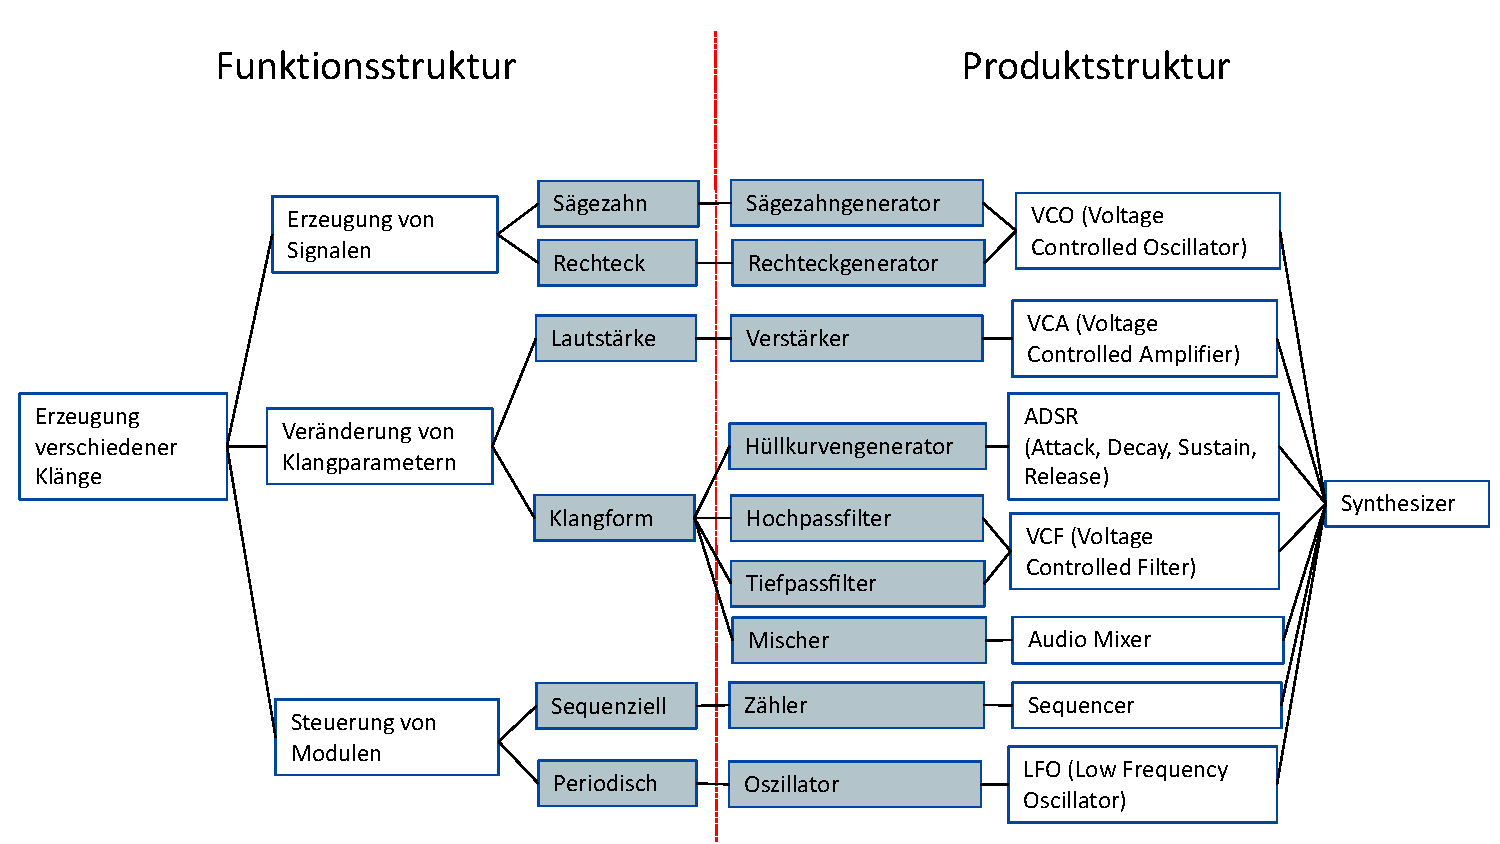
\includegraphics[width=0.8\textwidth]{figures/Produktarchitektur.pdf}}
	\caption{Produktarchitektur des modularen Synthesizers}
	\label{fig:fig:Produktarchitektur}
\end{figure}


\newpage
\section{Grundlegende analoge Prinzipien}
\label{sec:AnalogePrinzipien}






\chapter{Beispiele}\label{ch:method}
Im Folgenden werden abseits der reinen Subroutinen-Funktion alle Konstrukte mittels kurzer Beispiele erläutert. Die verwendete Python-Version ist hierbei ``3.9.7'' und diese wurde auf einem Windows-PC (64bit-Betriebssystem) mit IDLE ausgeführt. Die im Erklärtext beigefügten Zeilenangaben beziehen sich immer auf das jeweilige Beispielprogramm.
\section{Koroutinen}
\begin{lstlisting}[language=Python,caption={Beispiel f"ur die Verwendung von Koroutinen},captionpos=b]
def summierFunktion_2():
    print(``Warte auf Werte..'')
    while True:
        parA = (yield)
        parB = (yield)     
        summe = int(parA) + int(parB)    
        print(int(summe))

#Aufruf der Koroutine
summierer = summierFunktion_2()
        
#Ausfuehren der Koroutine bis zum ersten "yield"-Ausdruck
summierer.__next__()

#Senden der Parameter
summierer.send(35)
summierer.send(12)

#Schliessen der Koroutine
summierer.close()        
\end{lstlisting}

Wird das Programm ausgeführt, passiert beim Aufruf von ``summierFunktion\textunderscore 2'' noch nichts. Erst mit dem Befehl ``summierer.\textunderscore\textunderscore next\textunderscore\textunderscore ()'' (Z. 13) gibt die Funktion den ``print''-Befehl (Z. 2) und rückt bis zum ersten Auftreten des Schlüsselwortes ``yield'' vor. Mittels ``summierer.send'' (Z. 16-17) können Werte, in diesem Fall die Ganzzahlen 35 und 12, übermittelt werden. Diese Zahlen werden anschließend von den ``(yield)''-Aufrufen (Z. 4-5) an die lokalen Variablen der Funktion übergeben. Wichtig ist hierbei ist, die Reihenfolge nach dem FIFO-Prinzip zu beachten. Im Beispiel der Addition spielt diese zwar keine Rolle, aber in anderern Applikationen kann dies entscheident sein. Nach Erhalt beider Zahlen wird der Rest der Funktion ausgeführt und das Ergebnis der Addition wird ausgegeben (Z. 7). Im vorher genannten Beispiel ergibt dies den Wert ``47''. Würde die Koroutine nicht mittels ``summierer.close'' (Z. 20) geschlossen werden, könnte man weiterhin neue Zahlen an ``summierer'' senden.\\
Die exemplarische Darstellung der Koroutinen-Funktionalität macht sehr deutlich, wie nützlich und unkompliziert die Verwendung dieses Konstruktes ist. Abseits dieses Verwendungsbeispiels wären auch komplexere Erzeuger-Verbraucher-Strukturen möglich, bei denen mehrere Koroutinen, in einer Kette eingereiht oder parallel aufgebaut, Daten austauschen können.

\section{Threads}
\begin{lstlisting}[language=Python,caption={Beispiel f"ur die Verwendung von Threads},captionpos=b]
import threading
import time

neueZahlenWerte = False
neueSumme = False
summiererAktiv = True
zahlA,zahlB,ergebnis = 0

def summmierFunktion_3():
    print(``Der Summierer wurde gestartet...'')
    global neueZahlenWerte, neueSumme, ergebnis
    
    while summiererAktiv:
       if neueZahlenWerte == True:
           neueZahlenWerte = False
           ergebnis = int(zahlA) + int(zahlB)
           neueSumme = True
            
if __name__ == "__main__":    
    print(``Starten des Threads im Hauptprozess...'')
    summierer = threading.Thread(target=summmierFunktion_3)
    summierer.start()

    zahlA = 3
    zahlB = 5
    neueZahlenWerte = True
    
    while neueSumme == False:
        time.sleep(1)
        print("...")
    
    print(f``Die errechnete Summe ist {ergebnis}!'')    
    summiererAktiv = False  
     
    summierer.join()
    print(``Summierer-Thread wurde beendet...'')
\end{lstlisting}
Mittels den Importieraufrufen (Z. 1-2) werden die Module ``threading'' und ``time'' eingebunden. 
``threading'' wird dabei für das komfortable Erstellen von Threads in einem Prozess benötigt \cite{PythonSoftwareFoundation.}.``time'' wird benötigt, um den ``time.sleep(1)''-Befehl verwenden zu können, welcher eine Wartezeit verursacht \cite{PythonSoftwareFoundation.c}. 
Da der Thread dauerhaft lauffähig ist und gleichzeitiges Zugreifen auf Variablen vermieden werden soll, muss zwischen Thread und Hauptprozess eine Synchronisation erfolgen. Dies wird über die globalen Variablen ``neueZahlenWerte'', ``neueSumme'' und ``summiererAktiv'' erreicht (Z. 4-6). Alternativ hätte man dies auch mit einem Semaphor-Objekt lösen können.
Mittels ``summierer $=$ threading.Thread(target $=$ summmierFunktion\_3)'' (Z. 21) wird ein Thread-Objekt mit entsprechendem Verweis auf die ``summierFunktion\_3()'' (Z. 9) erzeugt. 
Über den Befehl ``summierer.start'' (Z. 22) wird der Thread dann gestartet. Darauf hin ist der Thread lauffähig und die Funktion wird bis zur While-Schleife (Z. 13) abgearbeitet. Solange über die globale Variable ``neueZahlenWerte'' (Z. 14) keine Signalisierung neuer Werte übermittelt wird, findet kein Vorrücken statt. Bei Freigabe durch Setzen der ``neueZahlenWerte''-Variable werden erst die Variablen ``parA'' und ``parB'' zu einer Summe addiert und anschließend mittels Setzen der Variable ``neueSumme'' das Ende der Rechenoperation signalisiert (Z. 16-17). Der Hauptprozess hat mittels aktiven Wartens auf die Freigabe mit der Fortführung pausiert (Z. 28-30). Ist die Freigabe erteilt wird mit der Ausführung fortgefahren und das Ergebnis der Rechnung ausgegeben (Z. 32). Um die Endlosschleife des ``summierer''-Threads zu beenden, wird die Variable ``summiererAktiv = False'' gesetzt und mittels ``summierer.join()'' wird auf das Beenden des Threads gewartet (Z. 35).\\
Die vielfältigen Möglichkeiten, Threads einzusetzen, übersteigen bei weitem die Komplexität des gewählten Beispieles. Gerade im Bereich der Semaphoren kann mittles den Funktionen ``acquire()'' und ``release()'' sehr einfach eine Synchronisation zwischen Threads erreicht werden \cite{PythonSoftwareFoundation.}. Dies ermöglicht eine komfortable Kommunikation zwischen Threads per globaler Variablen, welche deutlich unkomplizierter ist als bei der Kommunikation von eigenständigen Prozessen.
\newpage
\section{Asyncio}
\begin{lstlisting}[language=Python,caption={Beispiel f"ur die Verwendung von Asyncio},captionpos=b]
import asyncio
import random
import time

async def summierFunktion_4(parA, parB):

        #asynchrones Warten mit variierender Wartezeit zwischen 1 und 5s
        wartezeit = random.randint(1,10)
        await asyncio.sleep(wartezeit)
        
        summe = int(parA) + int(parB)    
        return summe, wartezeit
        
async def async_main():
    #Aufrufen der Summier-Funktion mit versch. Werten
    ergebnis_liste = await asyncio.gather(\
    summierFunktion_4(5, 39),\
    summierFunktion_4(5, 46),\
    summierFunktion_4(78, 69))
    return ergebnis_liste
    
if __name__ == "__main__":
    #Starten der Zeitmessung und Aufruf der asynchronen Hauptroutine
    start_Zeit = time.perf_counter()
    ergebnisse = asyncio.run(async_main())
    #Errechnen der verstrichenen Zeit 
    end_Zeit = time.perf_counter()
    vergangene_Zeit = end_Zeit - start_Zeit
    
    i = 0       
    for elem in ergebnisse:
        i = i + 1
        print(f``Das Ergebnis der {i}ten Rechnung ist {elem[0]} \ 
        und die Wartezeit war {elem[1]}.'')

    print(f``Die Rechnung hat {vergangene_Zeit:0.2f} Sekunden gedauert.'')
\end{lstlisting}
\begin{lstlisting}[language=Python,caption={Ausgabe in IDLE bei Asyncio-Beispiel},captionpos=b]
Das Ergebnis der 1ten Rechnung ist 44 und die Wartezeit war 8.
Das Ergebnis der 2ten Rechnung ist 51 und die Wartezeit war 3.
Das Ergebnis der 3ten Rechnung ist 147 und die Wartezeit war 4.
Die Rechnung hat 8.01 Sekunden gedauert.
\end{lstlisting}
\newpage
In Auflistung 3.3 wird der Beispiel-Code für das ``asyncio''-Paket gezeigt. Mit ``summierFunktion\_4'' (Z. 5) und ``async\_main'' (Z. 14) werden zwei Funktionen mit dem ``async''-Schlüsselwort deklariert. 
In ``summierFunktion\_4'' wird, ähnlich wie in den vorherigen Beispielen, wieder ein Summieren zweier Werte ausgeführt (Z. 11), jedoch mit dem Unterschied, dass zusätzlich eine Wartezeit mittels des ``asyncio.sleep''-Befehls eingebunden wird (Z. 9). 
Dieser Befehl ist mit dem ``await''-Schlüsselwort gekennzeichnet. und bewirkt, dass nach Aufruf die derzeitige Summierroutine pausiert wird und eine andere angefangen bzw. fortgesetzt werden kann. 
Nach Ablauf der Wartezeit kann zur ursprüngliche Routine zurückgekehrt werden. ``summierFunktion\_4'' liefert neben dem Ergebnis der Rechnung auch die Wartezeit zurück, um anschließend die Effizienz des Programmes besser nachvollziehen zu können.
In ``async\_main'' werden mehrere Aufrufe der ``summierFunktion\_4'' mit verschiedenen Werten mittels ``asyncio.gather'' getätigt (Z. 16-19). Auch hier wird zum Ende der Funktion das Ergebnis in Form einer Liste zurückgegeben (Z. 20). Um später die Dauer der Ausführung von ``async\_main'' (Z. 25) besser interpretieren zu können, wird die Start- (Z. 24) und Endzeit (Z. 27) gespeichert \cite{PythonSoftwareFoundation.c}. Es wird sowohl das Ergebnis der Rechnung als auch die eingebaute Wartezeit in IDLE ausgegeben (Z. 30-34). Das Skript endet mit der Ausgabe der verstrichenen Zeit (Z. 36).
\\Die Ausgabe von IDLE ist in Auflistung 3.4 dargestellt. Wenig verwunderlich ist, dass die errechnete Summe in allen drei Fällen richtig ist. Weitaus interessanter sind jedoch die Wartezeiten. Hätte man die Summierfunktionen sequentiell ausgeführt, läge die verstrichene Zeit weit höher. Im Falle der gegebenen Wartezeiten wäre diese bei etwa 15 Sekunden. Diese Zahl ergibt sich aus der Addition der drei Zeiten. In der asynchronen Version haben wir hingegen eine gesamte Dauer von 8,01 Sekunden. Dies verdeutlicht auf einfache Weise, wie günstig sich die Verwendung von ``asyncio'' auf die Ausführdauer auswirken kann. Die etwa acht Sekunden enstehen, weil die Wartezeit der ersten Rechnung dieser entspricht und beim ``asyncio.gather'' (Z. 16) auf das Ende aller übergebener Funktionen gewartet wird. Alle anderen Rechenoperation werden während dieser acht Sekunden abgeschlossen und die erste erst nach Ablauf der Wartezeit \cite{PythonSoftwareFoundation.b}. 
\chapter{Fazit}\label{ch:fazit}
Mit den in der Studienarbeit vorgestellten Konzepten, Koroutine, Thread und Asyncio werden sehr nützliche Verfahren angeboten. Sie ermöglichen dem Python-Programmierer parallelartig arbeitende Programme zu entwickelen, um sich von der starren Struktur des sequentiellen Ablaufes zu lösen.
Mit den aufgeführten Beispielen konnte der Ablauf und auch die zu implementierende Struktur der Konzepte aufgezeigt werden. Neben den Threads, welche im Allgemeinen recht bekannt und verbreitet sind, erweisen sich gerade die Koroutine bzw. Asyncio als sehr nützlich. 
Besonders die Verwendung des kooperativen Multitaskings macht diese Verfahren robust gegenüber Zugriffsfehlern, welche bei Threads ohne Synchronisation sehr leicht auftreten können. 
Der zeitliche Vorteil, der beim Einsatz dieser Pakete entstehen kann, ist bei Asyncio deutlich sichtbar und auch leicht nachvollziebar. Vorsicht und bedachtes Vorgehen sind jedoch geboten, da leicht unübersichtliche Situationen entstehen können.



% remove if not needed
\appendix
%\chapter{Supplemental Information}\label{app:supplemental-information}

\Blindtext



\backmatter

\lstlistoflistings
\cleardoublepage

\printbibliography

\end{document}
